\section{Video Transcoder}
\label{sec:video_transcoder}


Terminato il processo di upload appena descritto inizia la fase di transcodifica, il video appena caricato su S3 viene preso in carico dal servizio di Elastic Transcoder, processato e in output si avrà un file con formato .m3u8 che permette quindi lo streaming HLS con i vantaggi illustrati nei capitoli precedenti. L’idea alla base e il funzionamento generale si evince dall’immagine seguente dove vediamo il flusso che parte da il Bucket S3 passa per una TranscodingPipeline dove il video viene convertito e nuovamente caricato su S3. 

\begin{figure}[htb]
 \centering
 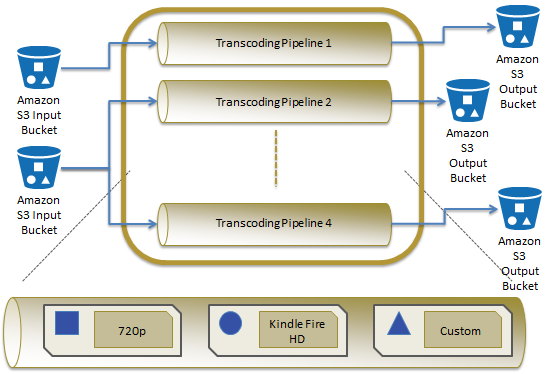
\includegraphics[width=1.0\linewidth]{images/chapter6/elastic_transcode_model.png}\hfill
 \caption[The Elastic Transcoder Model]{The Elastic Transcoder Model}
 \label{fig:fourV}
\end{figure}

Entrando nel dettaglio la transcodifica inizia al termine del MultipartUpload quando il server chiama API PUT /transcoders/createJob che prende in input i seguenti paramteri :
\begin{itemize}
      \item file\_name ovvero il file name che deve essere preso dal bucket per poi essere trasformato
      \item path ovvero il percorso remoto su cui effettuare lo storage quando termina la transcodifica
  \end{itemize}

 Tale API inizia la comunicazione con il servizio di ElasticTranscoder e crea quindi un nuovo JOB che verra inserito nella Pipeline specificata nel campo PipelineId.
\begin{lstlisting}[language=html]
  
Transcoder.createJob = function (file_name,path,callback){
    var input_params = {
      Input: { 
        Key: file_name, 
        FrameRate: 'auto', 
        Resolution: 'auto', 
        AspectRatio: 'auto', 
        Interlaced: 'auto', 
        Container: 'auto' 
      }, 
      PipelineId: PIPELINE_ID, // specifies output/input buckets in S3 
      OutputKeyPrefix: path,
      Output: { 
        Key: file_name, 
        PresetId: PRESET_ID, // specifies the output video format
        SegmentDuration: '5',
        ThumbnailPattern:'image/' + file_name + '-{count}'//modifica preset per determinare il numero di immagini
      },

    };    
    elastictranscoder.createJob(input_params, function(err, data) {
      if (err) {
        console.log(err, err.stack); // an error occurred
        callback(err);
        return;
      }else{
        callback(null, data);
      }
    });
  };
  
  Transcoder.remoteMethod('createJob', {
    http: { verb: 'put' },
    accepts: [
      {arg: 'file_name', type: 'string'},
      {arg: 'path', type: 'string'}
    ],
    returns: {arg: 'dataId', type: 'string'}
  });
\end{lstlisting}

Nel seguente codice è possibile vedere come il server nella richiesta specifica un PiepelineId ovvero un ID corrispondente a una determinata Pipeline dove il job in questione verra inserito.Un altro dato necessario richiesto dalle API è il PresetId che invece rappresenta ID del Preset che come già accennato nel capitolo 4 rappresenta are templates that contain most of the settings for transcoding media files from one format to another.
l’immagine seguente mostra la pipeline utilizzata durante la fase di test della piattaforma di X-learning come è possibile notare, il servizio di ElasticTranscoder mette a disposizione anche  servizi di notifica.

\begin{figure}[htb]
 \centering
 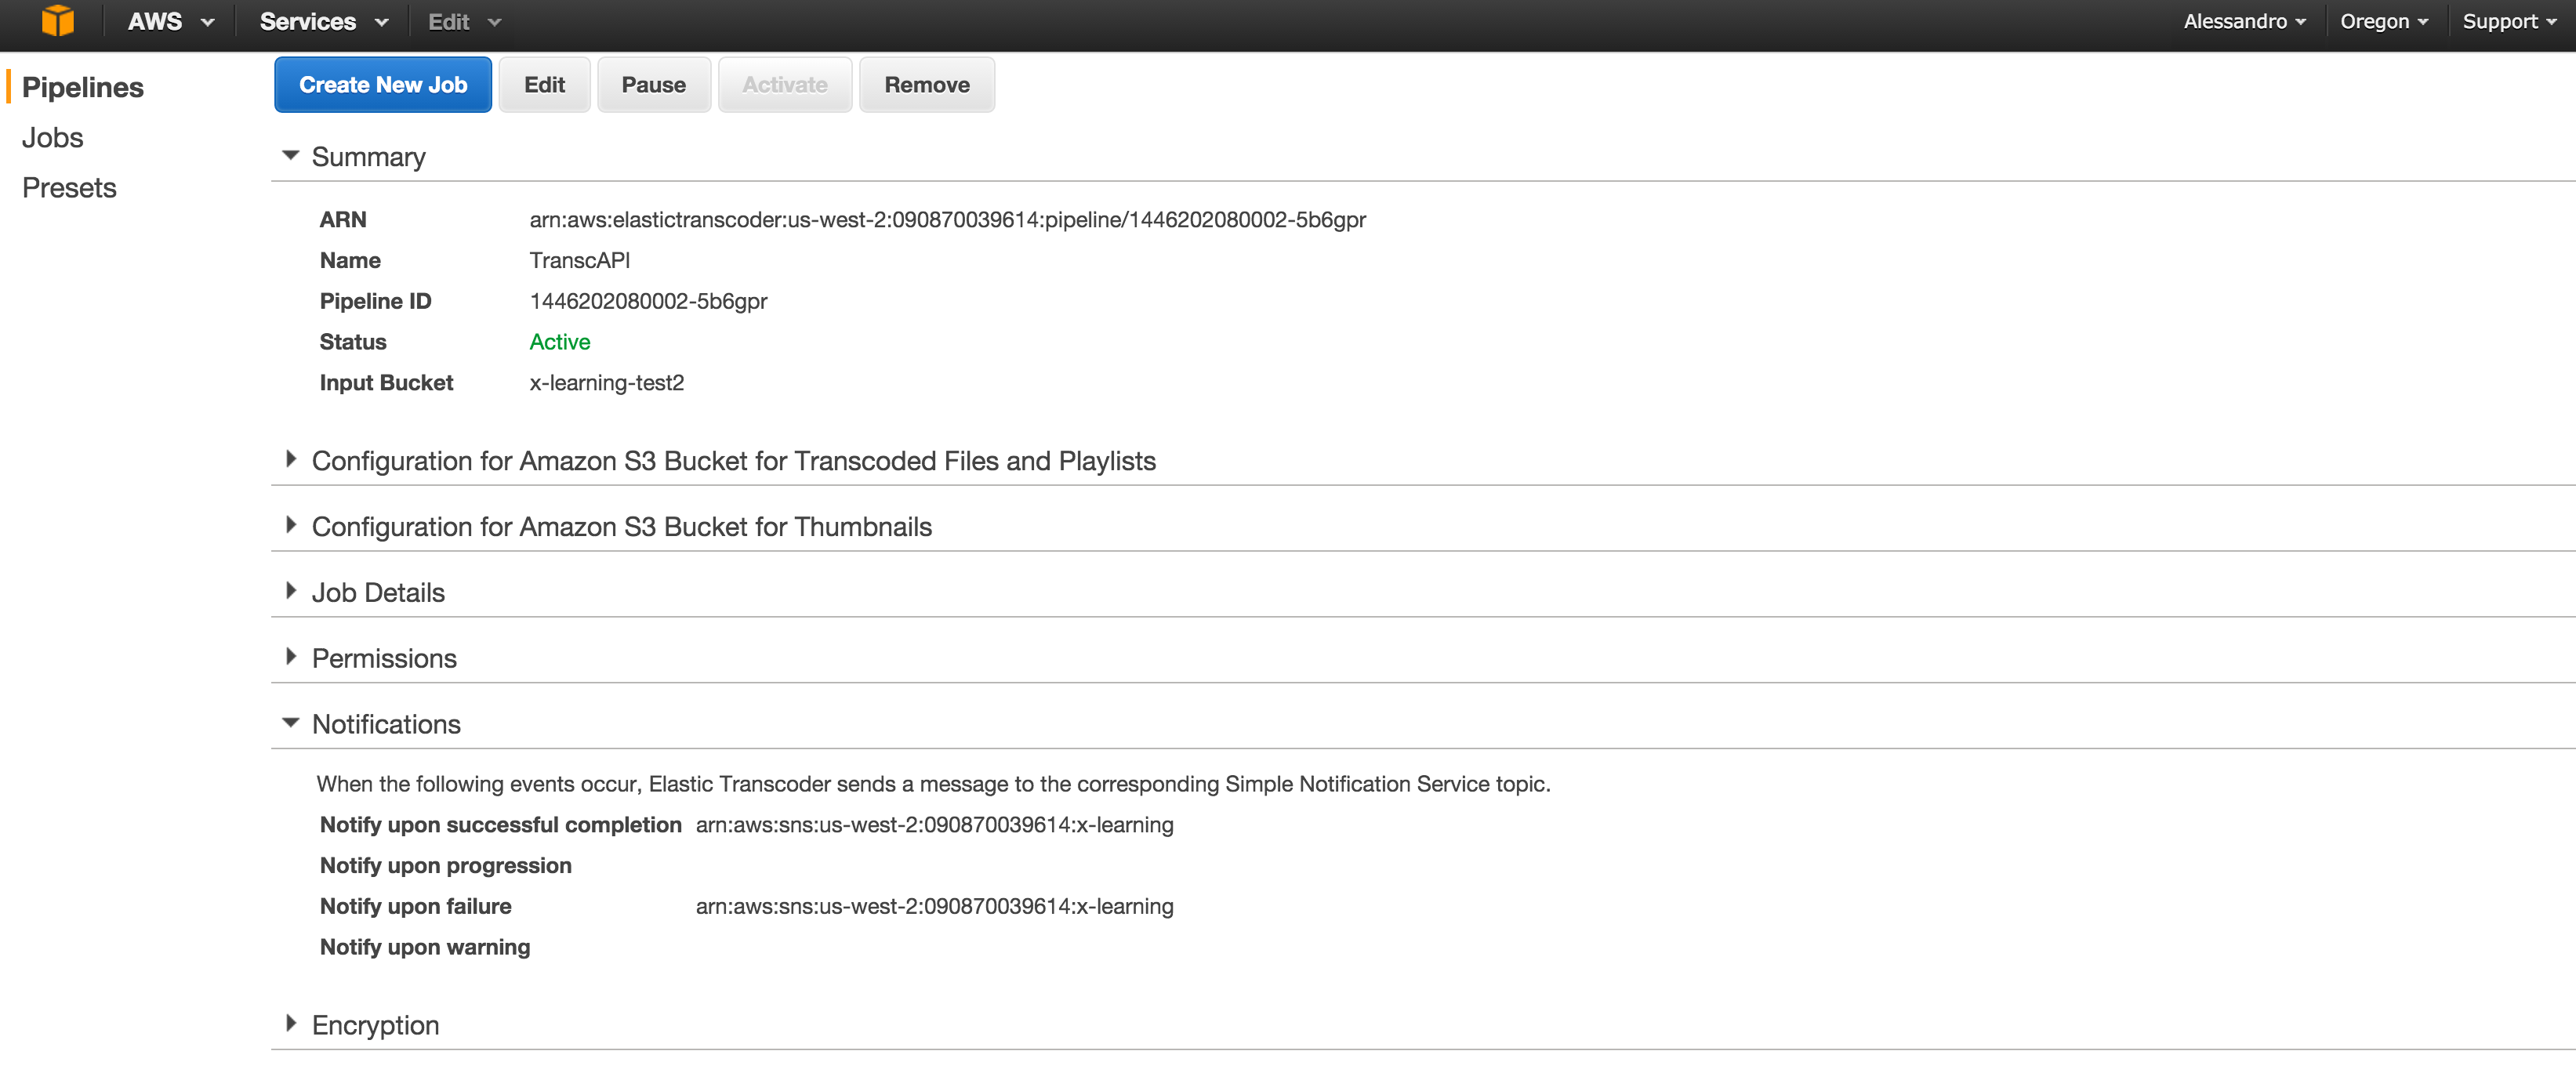
\includegraphics[width=1.0\linewidth]{images/chapter6/elastic_pipeline.png}\hfill
 \caption[Web Components]{Video upload}
 \label{fig:fourV}
\end{figure}
